در این فصل به ارائه‌ی برخی کارهای پیشین و مرتبط به موضوع این پژوهش خواهیم پرداخت. در مورد هر یک از این موارد به ارتباط آن با بحث جاری، کاربرد و یا نقاط تأثیرگذار آن در موضوع این پژوهش و هم‌چنین ضعف ها و نقایص آن‌ها پرداخته شده است. 
\section{الگوهای برنامه‌نویسی بازیگر}
\label{section:actorPatterns}
در برنامه‌نویسی همروند با بازیگر‌ها دو نوع الگوی کلی معرفی شده است \cite{Agha1990}: یکی  \textit{\gls{تقسیم-و-حل}}\LTRfootnote{devide and conquer} و دیگری \textit{\gls{خط لوله}}\LTRfootnote{pipeline}. 
در روش تقسیم-و-حل مسئله‌ی مورد بحث به زیربخش‌های کوچکتر و مستقل تقسیم می‌شود که هرکدام به صورت مستقل حل می‌شوند و نتایج هر زیربخش برای نتیجه‌گیری کلی ادغام می‌شوند. در برنامه‌نویسی به مدل بازیگر، برای پیاده‌سازی این الگو یک بازیگر رئیس\LTRfootnote{master} در نظر گرفته می‌شود که تعدادی بازیگر کارگر\LTRfootnote{worker} را برای حل زیربخش‌های مسئله ایجاد می‌کند. عمل تقسیم به وسیله‌ی فرستادن پیغام‌ حاوی حالت لازم برای حل زیر بخش به کارگر‌ها انجام می‌شود. کارگرها به نوبه‌ی خود منطق لازم برای حل زیر بخش را ایجاد نموده و نتیجه را به صورت پیغام دیگری برای بازیگر رئیس ارسال می‌کنند. نهایتا رئیس با ادغام نتایج جواب نهایی 
مسئله را تولید می‌کند. شایان ذکر است که فازهای تقسیم و حل لزوما توسط بازیگر یکسان اجرا نمی‌شوند. ممکن است اجرای فاز حل به بازیگر دیگری سپرده شود.\cite{Feng08scalablemodels}
مثال دیگری از پیاده‌سازی الگوی تقسیم-و-حل در مدل بازیگر  در \cite{Feng08scalablemodels} آمده است که در آن الگوریتم جستجوی سریع\LTRfootnote{quick sort} توسط این الگو پیاده شده است.
\begin{figure*}
    \begin{center}
	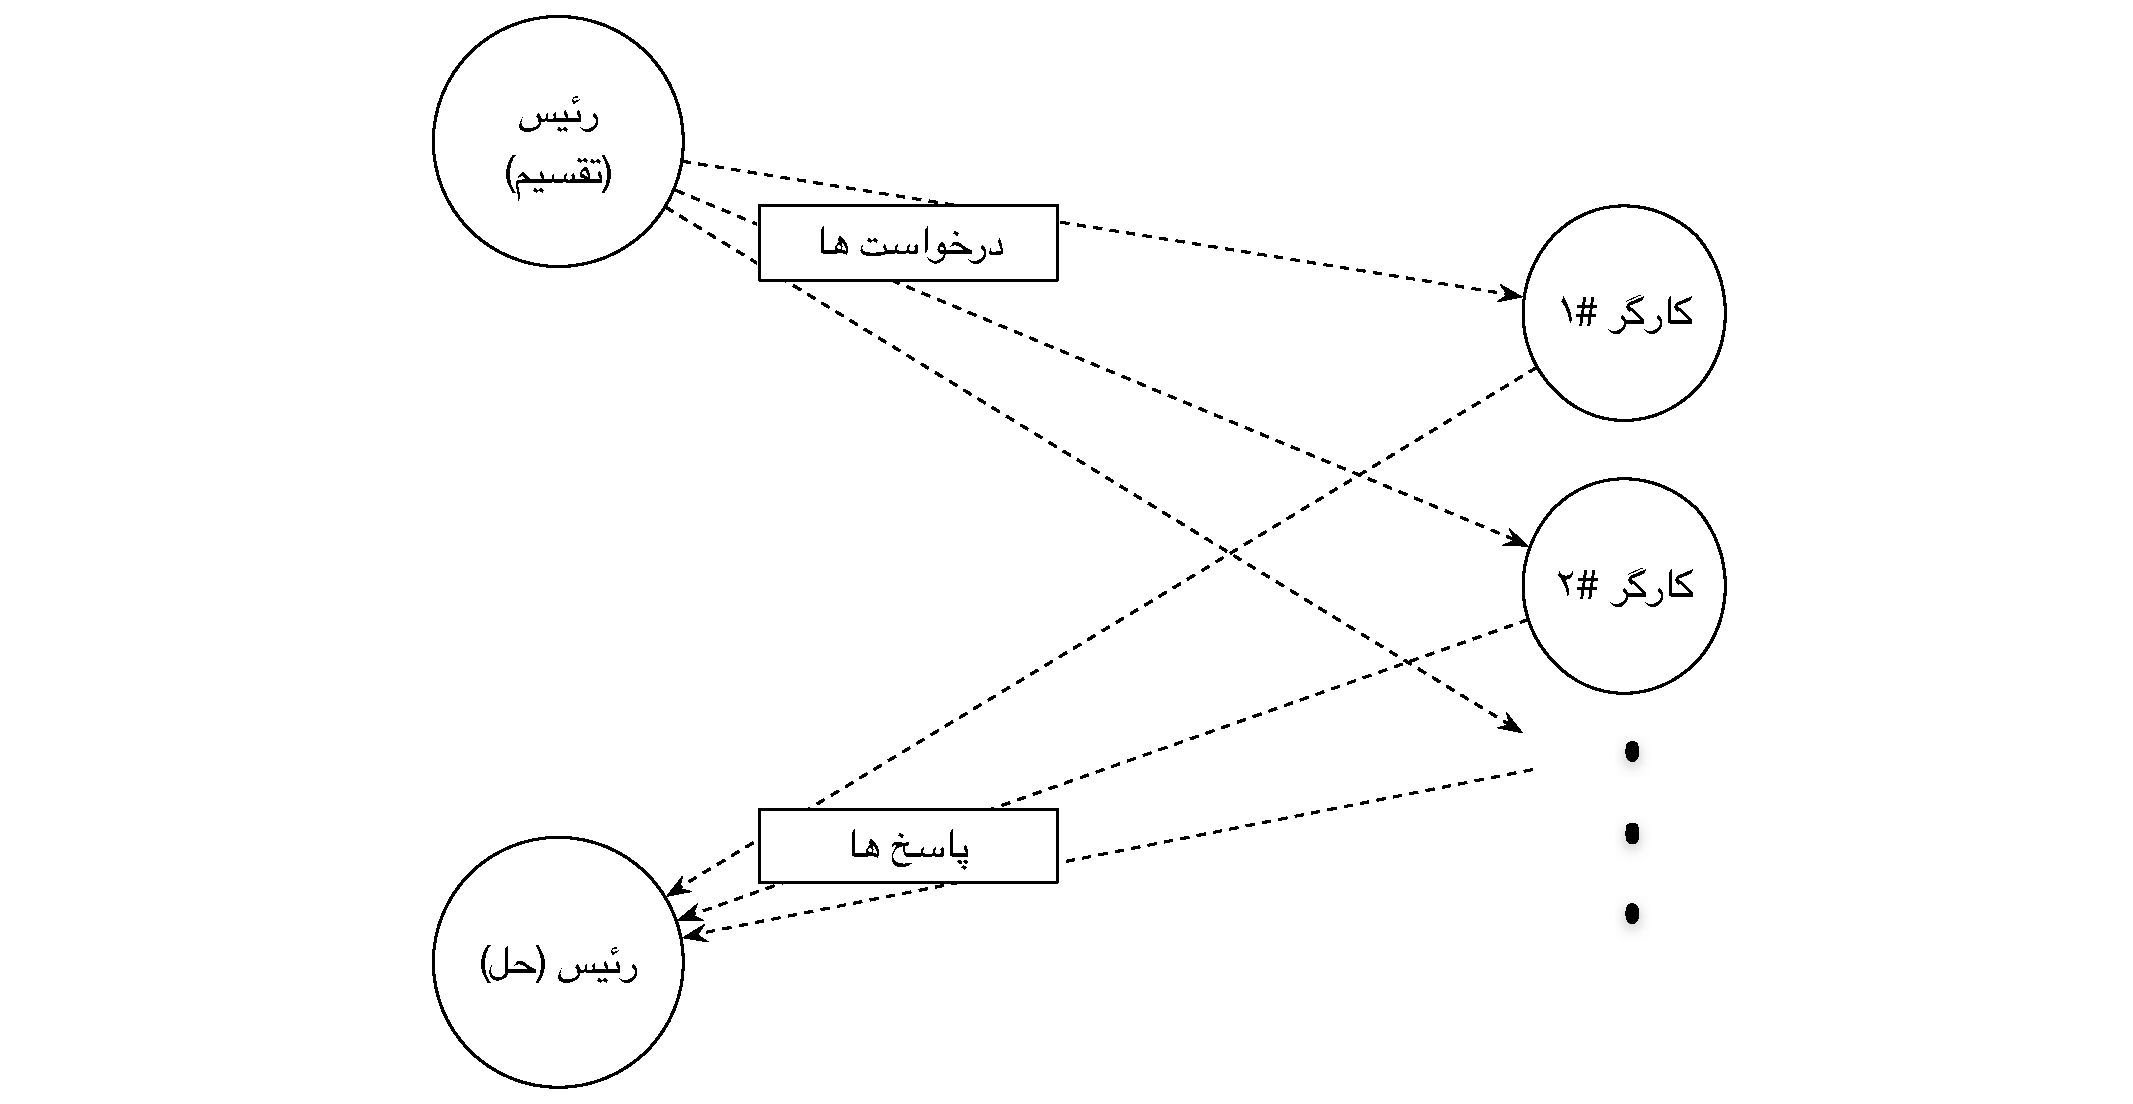
\includegraphics[width=16cm]{3-RelatedWork/Figures/Divide_and_Conquer.pdf}
    \end{center}
    \caption{\label{fig:divide_conquer}  شمای کلی از الگوی تقسیم-و-حل در مدل بازیگر }
\end{figure*}
شکل \ref{fig:divide_conquer} شمایی از نحوه‌ی پیاده‌سازی الگوی تقسیم-و-حل در مدل بازیگر را نمایش می‌دهد.\\
الگوی خط لوله برای حالت‌هایی مناسب است که فعالیت قابل تقسیم به بخش‌های افزایشی باشد. در این صورت هر بازیگر تغییرات مربوطه را در مدل ایجاد می‌کند و آن را به عنوان پیغام به بازیگر بعدی در خط لوله منتقل می‌کند.

\begin{figure*}
    \begin{center}
	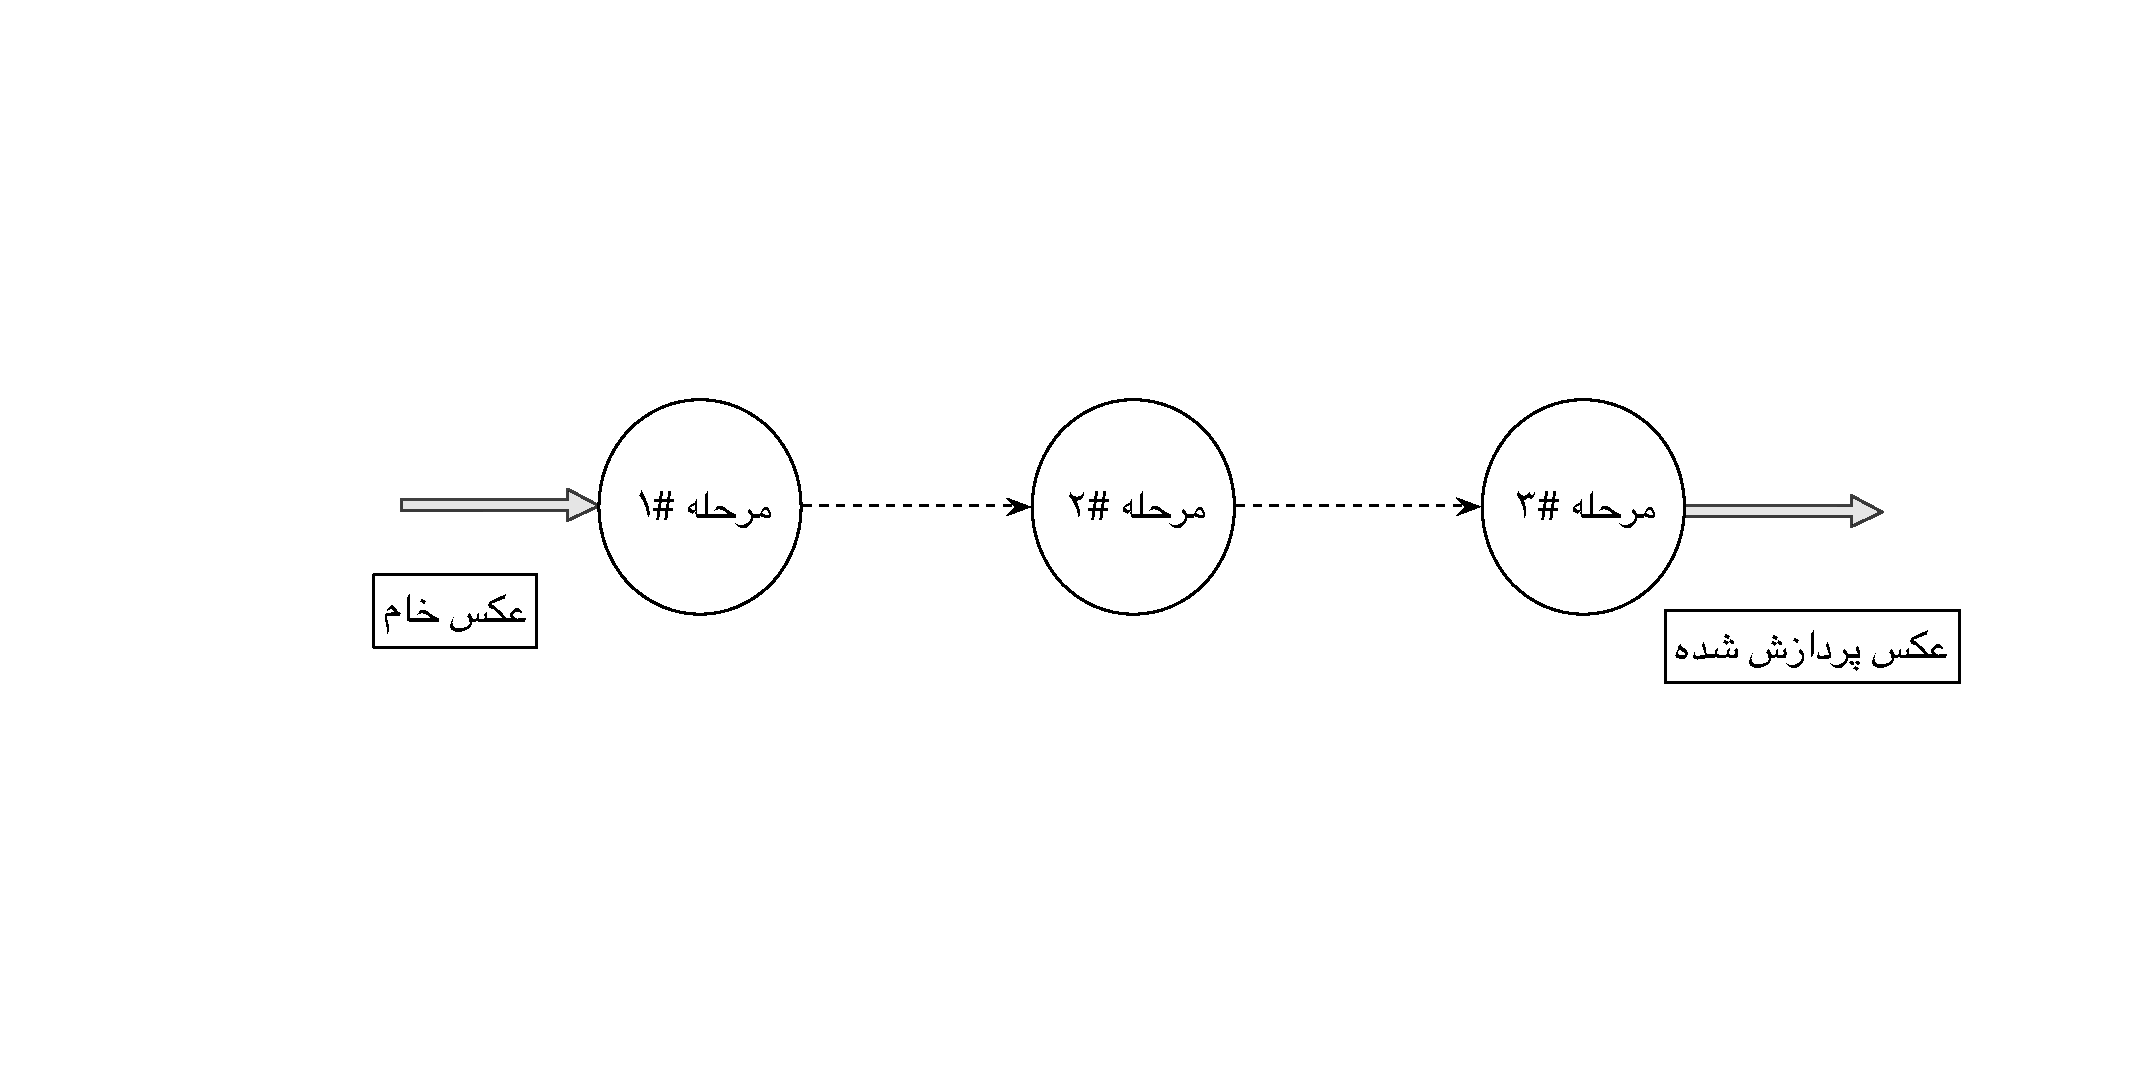
\includegraphics[width=16cm]{3-RelatedWork/Figures/pipeline.pdf}
    \end{center}
    \caption{\label{fig:pipeline}  مثالی از الگوی خط لوله (پردازش تصویر) }
\end{figure*}
به عنوان مثالی از الگوی خط لوله یک برنامه‌ی پردازش تصویر را در نظر بگیرید. هر مرحله از خط لوله، تغییراتی را در تصویر دریافتی ایجاد می‌کند و تصویر نتیجه را به مرحله‌ی بعد منتقل می‌کند. در پیاده‌سازی با روش بازیگر، هر مرحله به صورت یک بازیگر مدل می‌شود و تصویر به صورت پیغام بین مراحل رد و بدل می‌شود. در شکل \ref{fig:pipeline} شمایی از این الگو نشان داده شده‌ است. \\
در پژوهش‌های انجام شده مشخص شد که الگوهای ارائه شده صرفا الگوهای کلی همروندی هستند و جزئیات این الگوها در طراحی منطق دامنه، نحوه‌ی طراحی پیغام‌ها بررسی نشده اند .

\section{الگوهای همگام سازی}
\label{section:coordinationPatterns}
دسته‌ای از پژوهش‌های مرتبط با پژوهش جاری به بررسی  
\section{طراحی به روش ارتباط ناهمگام}
\label{section:asyncDesign}
سلام
\subsection{برناه‌نویسی موازی}
سلام